\section{gprof}

To install, as root, do
\begin{console}[fontsize=\footnotesize]
dnf install -y binutils
\end{console}

Create directory \verb!gprof/! and in this directory write
\VerbatimInput[frame=single,fontsize=\footnotesize]{../gprof/main.cpp}
Compile and link using \gpp\ but remember to include \verb!-pg! for both:
\begin{console}[fontsize=\footnotesize]
g++ main.cpp -pg -c -o main.o
g++ -pg main.o -o main.exe
\end{console}
or just
\begin{console}[fontsize=\footnotesize]
g++ main.cpp -pg -o main.exe
\end{console}

To run \verb!gprof!, do
\begin{console}[fontsize=\footnotesize]
gprof main.exe gmon.out > gprof.txt
\end{console}
You will get the file \verb!grof.txt! which looks something like
this (truncated on the right):
%\pyc{from pyutil import *;
%s = readfile('../gprof/gprof.txt');
%lines = s.split('\n');
%lines = [x[:90] for x in lines];
%s = '\n'.join(lines);
%writefile('../gprof/gprof-trunc.txt', s)
%}  
\VerbatimInput[frame=single,fontsize=\scriptsize]{../gprof/gprof-trunc.txt}
The report is made up of the \lq\lq flat profile" and the \lq\lq call graph".

The \lq\lq flat profile" is very easy to read.
Explanation is at the end of this section.

The \lq\lq call graph" part of the report allows you to see the function
call graph.
The call graph part is made up of sections.
Each section looks like this:
\begin{console}[fontsize=\footnotesize]
index % time  self  children  called
                                            f
                                            g
[5]                                     h   
                                            i
                                            j
                                            k
\end{console}
This is the section for function \verb!h! which is given an index of 5.
\verb!h! is called by \verb!f! and \verb!g!, and
\verb!h! calls \verb!i!, \verb!j!, \verb!k!.
Under the \verb!called! column, if you see
\begin{console}[fontsize=\footnotesize]
index % time  self  children  called
[5]                           5         h   
\end{console}
this means \verb!h! is called 5 times.
If you see
\begin{console}[fontsize=\footnotesize]
index % time  self  children  called
[5]                           1+4       h   
\end{console}
it means \verb!h! is recursive and there is 1 non-recursive call to
itself and there are 4 recursive calls.
If you see
\begin{console}[fontsize=\footnotesize]
index % time  self  children  called
                              2/5           g  
[5]                                     h   
\end{console}
this means \verb!g! calls \verb!h! 2 times out of a total of 5 functions calls
that \verb!g! makes.
If you see
\begin{console}[fontsize=\footnotesize]
index % time  self  children  called
[5]                                     h   
                              10/20         i
\end{console}
this means \verb!h! calls \verb!i! 10 times out of a total of 20 times
\verb!i! is called.

Warning: If the total runtime is very small, the report might be empty.


\begin{ex}
  \mbox{}
  \begin{myenum}
  \item
    There's a \verb!std::swap! function from \cpp\ STL.
    Run \verb!gprof! on your program after changing your \verb!swap! to
    \verb!std::swap! in the bubblesorting progam.
    Which swap function is faster, \verb!swap! or \verb!std::swap!?
  \item
    Write another version of the bubblesort program using
    arrays instead of \verb!std::vector!.
    Generate a new \verb!gprof! report.
    Which version is faster?
  \end{myenum}
\end{ex}
 

\begin{ex}
  Write a program where \verb!main()! calls a recursive function
  \verb!f()!.
  To make sure \verb!f()! actually takes
  some time to execute, insert some redundant time intensive
  loop inside \verb!f()!
  (otherwise the total time taken is too small and no
  \verb!gprof! report is generated).
  Generate a \verb!gprof! report and make sure you can read it.
  \qed
\end{ex}

\begin{ex}
  Write a quicksort program, writing as many functions as you can.
  You should of course have a function to select the pivot (use
  median-of-three) and a function to perform partitioning.
  Generate a \verb!gprof! report and read it carefully.
\end{ex}

If you want to draw a graph representation of the function call information
in a \verb!gprof! report,
you can use gprof2dot which uses \verb!graphviz! (see CISS350, etc.)
To install \verb!grof2dot!, as root, do
\begin{console}[fontsize=\footnotesize]
dnf install -y gprof2dot
\end{console}
Exit root.
To generate a dot file do
\begin{console}[fontsize=\footnotesize]
gprof2dot gprof.txt > gprof.dot
\end{console}
You'll get a \verb!gprof.dot! file.
Next generate a jpg file:
\begin{console}[fontsize=\footnotesize]
dot -Tjpg gprof.dot -o gprof.jpg
\end{console}
You'll get \verb!gprof.jpg!:
\begin{center}
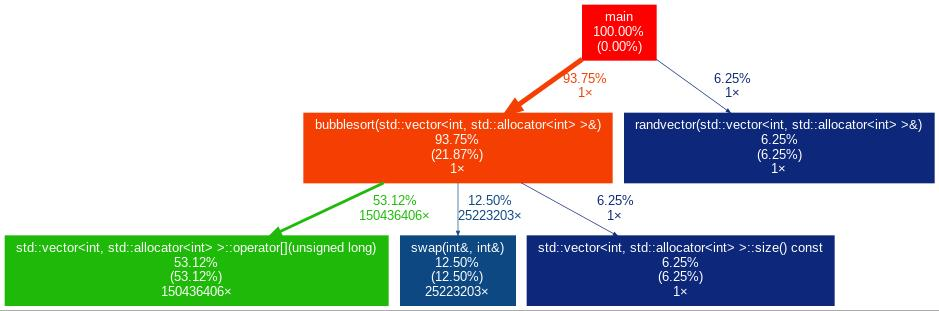
\includegraphics[width=\textwidth]{../gprof/gprof.jpg}
\end{center}

\begin{ex}
  Generate function call graph diagrams of your earlier sorting
  programs, 
  one for the program that uses arrays and another one that
  uses \verb!std::vector!.
  \qed
\end{ex}
